% KILT: accepting lasso in the product graph (figure for Sec. 2.2)
% Compile with:  pdflatex kilt_lasso.tex
% Uses the same colour names as kilt_cover.tex, so a palette change
% made there can be copied here unchanged.
\documentclass[tikz,border=12pt]{standalone}

\usepackage{amsmath,amssymb}
\usetikzlibrary{arrows.meta,calc}

% ---------- palette (identical names to kilt_cover.tex) ----------
\definecolor{navy}{HTML}{1F3A5F}
\definecolor{teal}{HTML}{2E7D86}
\definecolor{tealfill}{HTML}{EFF6F7}
\definecolor{mred}{HTML}{B4534D}   % muted red: counterexample only
\definecolor{mredfill}{HTML}{F8EDEC}

% ---------- shared styles ----------
\tikzset{
  >={Stealth[length=2.6mm,width=2.2mm]},
  trans/.style ={navy,line width=0.9pt,->,shorten >=1pt},
  cex/.style   ={mred,line width=1.5pt,->,shorten >=1pt},
  ghost/.style ={navy!35,line width=0.8pt,->,shorten >=1pt},
  pstate/.style={circle,draw=navy,fill=tealfill,line width=1pt,minimum size=1.75cm,
                 inner sep=0pt,align=center,font=\footnotesize\sffamily,text=navy},
  gstate/.style={pstate,draw=navy!40,fill=white,text=navy!55},
  hstate/.style={pstate,draw=mred,fill=mredfill,text=mred,line width=1.5pt},
  acc/.style   ={double distance=1.5pt},
  astate/.style={circle,draw=navy,fill=tealfill,line width=0.9pt,minimum size=1.1cm,
                 inner sep=0pt,font=\footnotesize,text=teal},
  caption/.style={font=\scriptsize\sffamily\bfseries,text=teal},
  note/.style  ={font=\scriptsize,inner sep=1pt},
}
% automaton states are teal and maths-italic; system states are sans-serif
\newcommand{\q}[1]{\textcolor{teal}{\ensuremath{q_{#1}}}}

\begin{document}
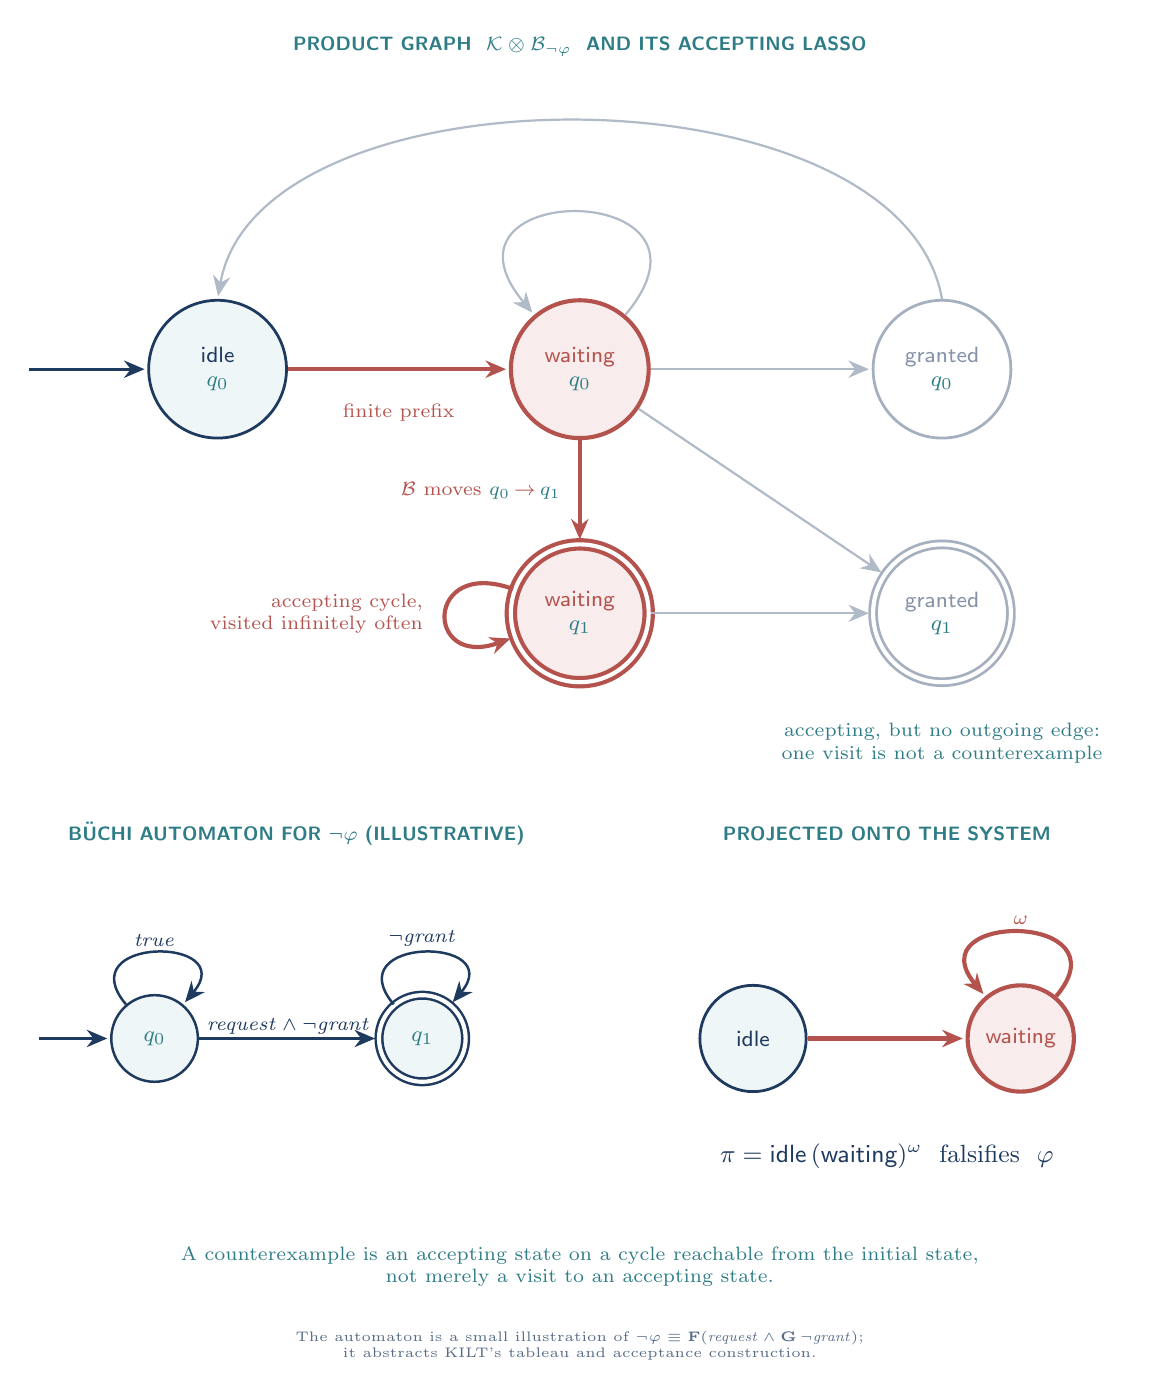
\begin{tikzpicture}

%% =====================================================
%% (a) PRODUCT GRAPH  K x B_{not phi}
%% rows = automaton state, columns = system state
%% =====================================================
\node[caption] at (0,4.1) {PRODUCT GRAPH \ $\mathcal{K}\otimes\mathcal{B}_{\neg\varphi}$ \ AND ITS ACCEPTING LASSO};

\node[pstate]         (iq0) at (-4.6, 0)  {idle\\[-1pt]\q{0}};
\node[hstate]         (wq0) at ( 0,   0)  {waiting\\[-1pt]\q{0}};
\node[gstate]         (gq0) at ( 4.6, 0)  {granted\\[-1pt]\q{0}};
\node[hstate,acc]     (wq1) at ( 0,  -3.1){waiting\\[-1pt]\q{1}};
\node[gstate,acc]     (gq1) at ( 4.6,-3.1){granted\\[-1pt]\q{1}};

% initial product state
\draw[trans,line width=1.1pt] ($(iq0.west)+(-1.5,0)$) -- (iq0.west);

% ---- the lasso: finite prefix, then accepting cycle (red) ----
\draw[cex] (iq0) -- (wq0);
\draw[cex] (wq0) -- (wq1);
\draw[cex] (wq1.160) to[out=160,in=-160,looseness=5] (wq1.-160);

% ---- all other reachable product edges (faded) ----
\draw[ghost] (wq0.50)  to[out=50,in=130,looseness=5] (wq0.130);
\draw[ghost] (wq0) -- (gq0);
\draw[ghost] (wq0) -- (gq1);
\draw[ghost] (wq1) -- (gq1);
\draw[ghost] (gq0.north) to[out=100,in=80,looseness=0.85] (iq0.north);

% ---- annotations ----
\node[note,mred] at (-2.3,-0.55) {finite prefix};
\node[note,mred,anchor=east] at (-0.2,-1.55) {$\mathcal{B}$ moves \q{0}$\,\to\,$\q{1}};
\node[note,mred,align=right,anchor=east] at (-1.95,-3.1) {accepting cycle,\\visited infinitely often};
\node[note,teal,align=center] at (4.6,-4.75)
  {accepting, but no outgoing edge:\\one visit is not a counterexample};

%% =====================================================
%% (b) AUTOMATON  (illustrative)      (c) PROJECTION
%% =====================================================
\node[caption] at (-3.6,-5.9) {B\"UCHI AUTOMATON FOR $\neg\varphi$ (ILLUSTRATIVE)};
\node[astate]     (a0) at (-5.4,-8.5) {$q_0$};
\node[astate,acc] (a1) at (-2.0,-8.5) {$q_1$};
\draw[trans] ($(a0.west)+(-0.9,0)$) -- (a0.west);
\draw[trans] (a0) -- node[above,note,navy] {$\mathit{request}\wedge\neg\mathit{grant}$} (a1);
\draw[trans] (a0.130) to[out=130,in=50,looseness=4] node[above=1pt,note,navy] {$\mathit{true}$} (a0.50);
\draw[trans] (a1.130) to[out=130,in=50,looseness=4] node[above=1pt,note,navy] {$\neg\mathit{grant}$} (a1.50);

\node[caption] at (3.9,-5.9) {PROJECTED ONTO THE SYSTEM};
\node[pstate,minimum size=1.35cm] (pi) at (2.2,-8.5) {idle};
\node[hstate,minimum size=1.35cm] (pw) at (5.6,-8.5) {waiting};
\draw[cex] (pi) -- (pw);
\draw[cex] (pw.50) to[out=50,in=130,looseness=4]
  node[above=1pt,note,mred] {$\omega$} (pw.130);
\node[navy,font=\small,inner sep=0pt] at (3.9,-10.0)
  {$\pi=\textsf{idle}\,(\textsf{waiting})^{\omega}$ \ falsifies \ $\varphi$};

%% =====================================================
%% takeaway + footnote
%% =====================================================
\node[teal,font=\scriptsize,inner sep=0pt,align=center] at (0,-11.4)
  {A counterexample is an accepting state on a cycle reachable from the initial state,\\
   not merely a visit to an accepting state.};
\node[navy!75,font=\tiny,inner sep=0pt,align=center] at (0,-12.4)
  {The automaton is a small illustration of $\neg\varphi\equiv\mathbf{F}(\mathit{request}\wedge\mathbf{G}\,\neg\mathit{grant})$;\\
   it abstracts KILT's tableau and acceptance construction.};

\end{tikzpicture}
\end{document}
